\documentclass{article}

\usepackage[letterpaper, portrait, margin=1.5in]{geometry}

\usepackage{fancyhdr}
\usepackage{ragged2e}
\usepackage{graphicx}
\usepackage{caption}
\usepackage{amsmath}
\usepackage{rotating}

\usepackage{listings}
\usepackage{color}

\definecolor{dkgreen}{rgb}{0,0.6,0}
\definecolor{gray}{rgb}{0.5,0.5,0.5}
\definecolor{mauve}{rgb}{0.58,0,0.82}

\lstset{frame=tb,
  language=Java,
  aboveskip=3mm,
  belowskip=3mm,
  showstringspaces=false,
  columns=flexible,
  basicstyle={\small\ttfamily},
  numbers=none,
  numberstyle=\tiny\color{gray},
  keywordstyle=\color{blue},
  commentstyle=\color{dkgreen},
  stringstyle=\color{mauve},
  breaklines=true,
  breakatwhitespace=true,
  tabsize=4
}

\setcounter{secnumdepth}{1}

\usepackage{chngcntr}
\counterwithin{figure}{section}

\renewcommand*{\thepage}{C\arabic{page}}

\pagestyle{fancy}
\lhead{ACME Robotics}
\chead{\#8367}
\rhead{\ifcontents Contents \else Week \thesection \fi}

\newif\ifcontents
\contentstrue

\makeatletter
\renewcommand{\@seccntformat}[1]{}
\makeatother
\begin{document}
\subsection{Attend the Northern California Regional Championships}
The Northern California Regionals span two days. 56 teams from the Northern California League, which spans from Bakersfield to the California - Oregon border, compete for eight spots of advancement to Worlds. These eight winners are the winning alliance (consisting of three teams), then 2nd place alliance captain, 1st, 2nd, and 3rd place Inspire winners, and finally the Think award winner. That meant that ACME had to place high enough during the competition, or try to win Inspire or Think in order to qualify for the World Championship. \\

Judging and inspection began on Saturday and then match play on Sunday. Their judging presentation was at 4:30 in the afternoon on Saturday. Their judging presentation went very well! Then, they went and set up their pit area and took the robot to inspection (which they passed). \\

Sunday started bright and early with opening ceremonies and qualification matches. ACME played matches throughout the day and won 3 out 5 of them, placing them at 15th out of 28 teams in their division. During alliance selection they were picked to be on the third seed alliance. \\

During elimination rounds they made it to our division finals. This meant they played against the first seed alliance. The first seed alliance ultimately beat them, but it was very fun to compete in the finals. \\

Since they had not qualified through match play, they need to win one of the awards mentioned above. As each award passed, they became more and more discouraged as they hadn't been nominated for any. Then they announced the Think winner - and it was ACME Robotics! \\

The team was so excited and ran down the bleachers to high-five all of the tournament officials, referees, and judges. The Think award winner has a guaranteed spot at the World Championship and they couldn't believe they had received it! \\

They were so honored to have been given the Think award and are already planning their pit for the World Championship. \\

\subsection{Northern California Regional Championships retrospective}
The team finds it refreshing if they take a meeting to reflect on the tournament they just participated in, and talk about how they can make their next tournament experience better. They also take the time to write an action plan for the weeks in between tournaments. \\

The team has three different categories to place things in during the retrospective, which are each represented by a face. There is the good things, the okay things, and the not so great things that happened during the tournament. You can see a picture of ACME's retrospective as seen in Figure \ref{fig:retro}. \\

\begin{figure}
    \centering
    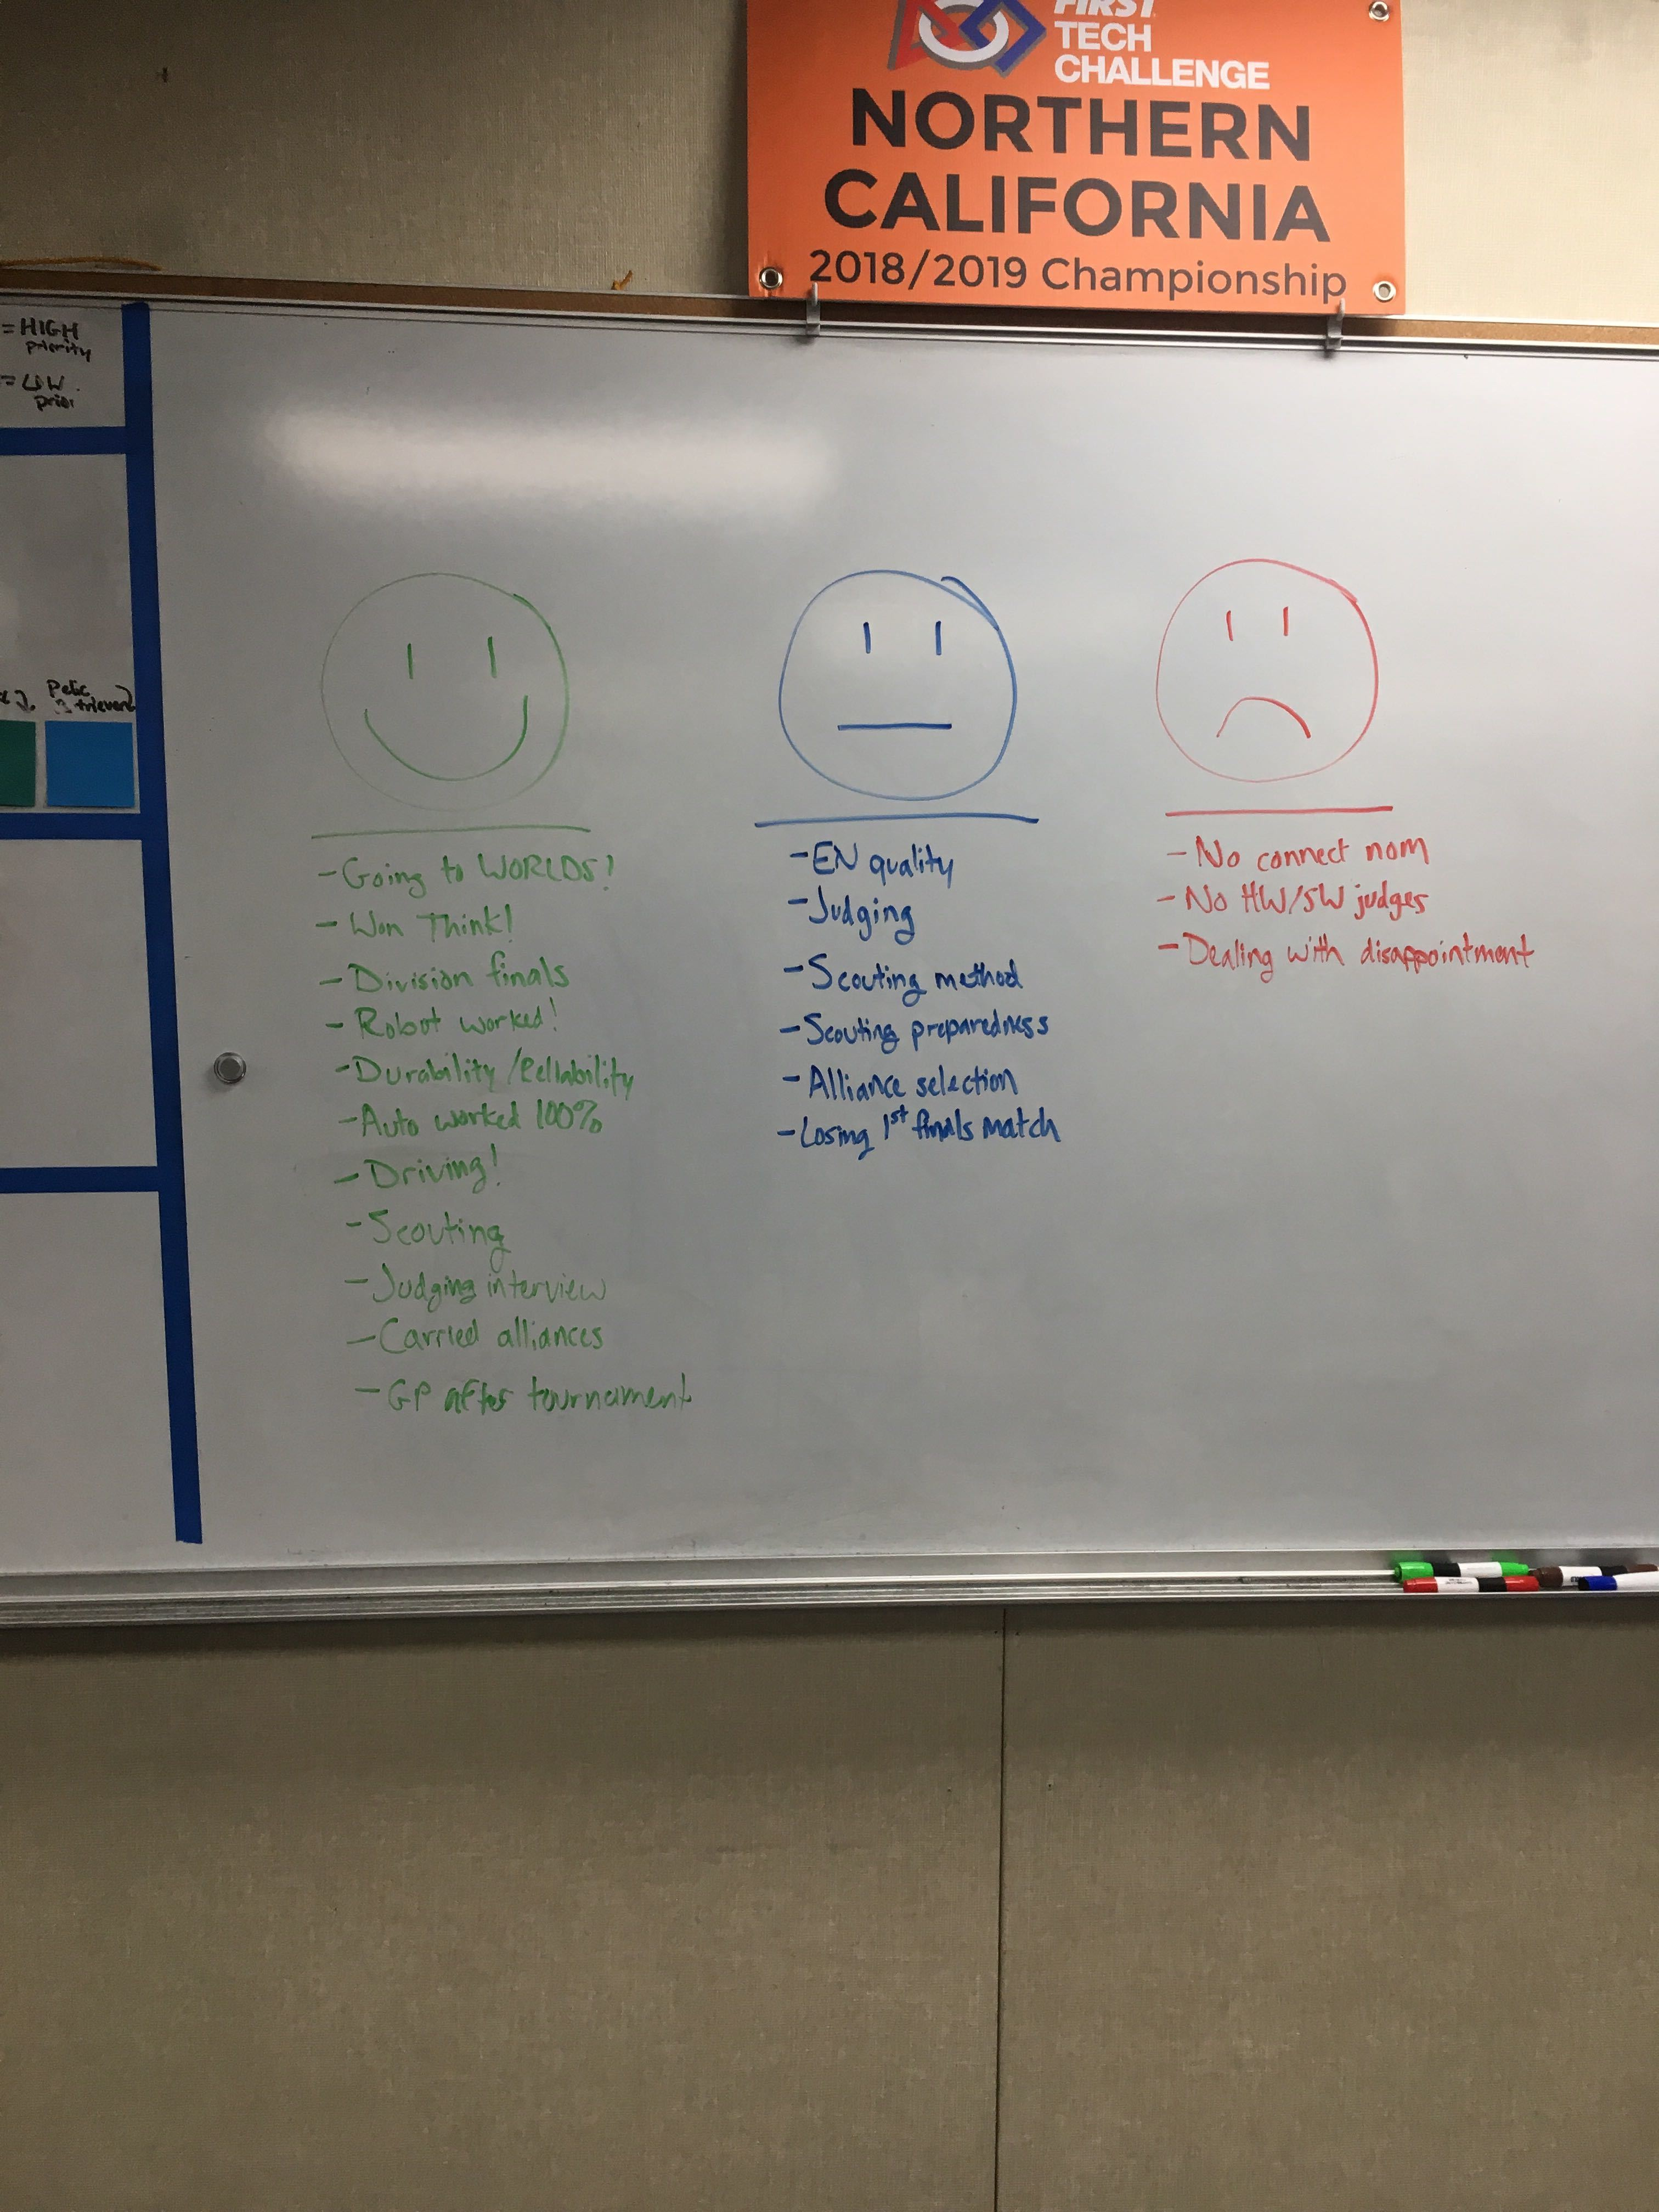
\includegraphics[width= 0.5 \textwidth]{27_03-04/images/retrospective.JPG}
    \caption{ACME's Retrospective}
    \label{fig:retro}
\end{figure}

ACME also has a tradition of making goals and action plans to complete before the next tournament. Since their next tournament would be Worlds, they decided to make Worlds goals as well. One of the top goals for this year is to have fun at Worlds. This was because the last time they went to Worlds, the team became very stressed and disappointed by the end of the week, and that wasn't a lot of fun. They have decided for this year they should take the time to have fun because they don't know if they will be back in Houston next year. You can see the rest of the goals and action plans in Figure \ref{fig:goals}. \\

\begin{figure}
    \centering
    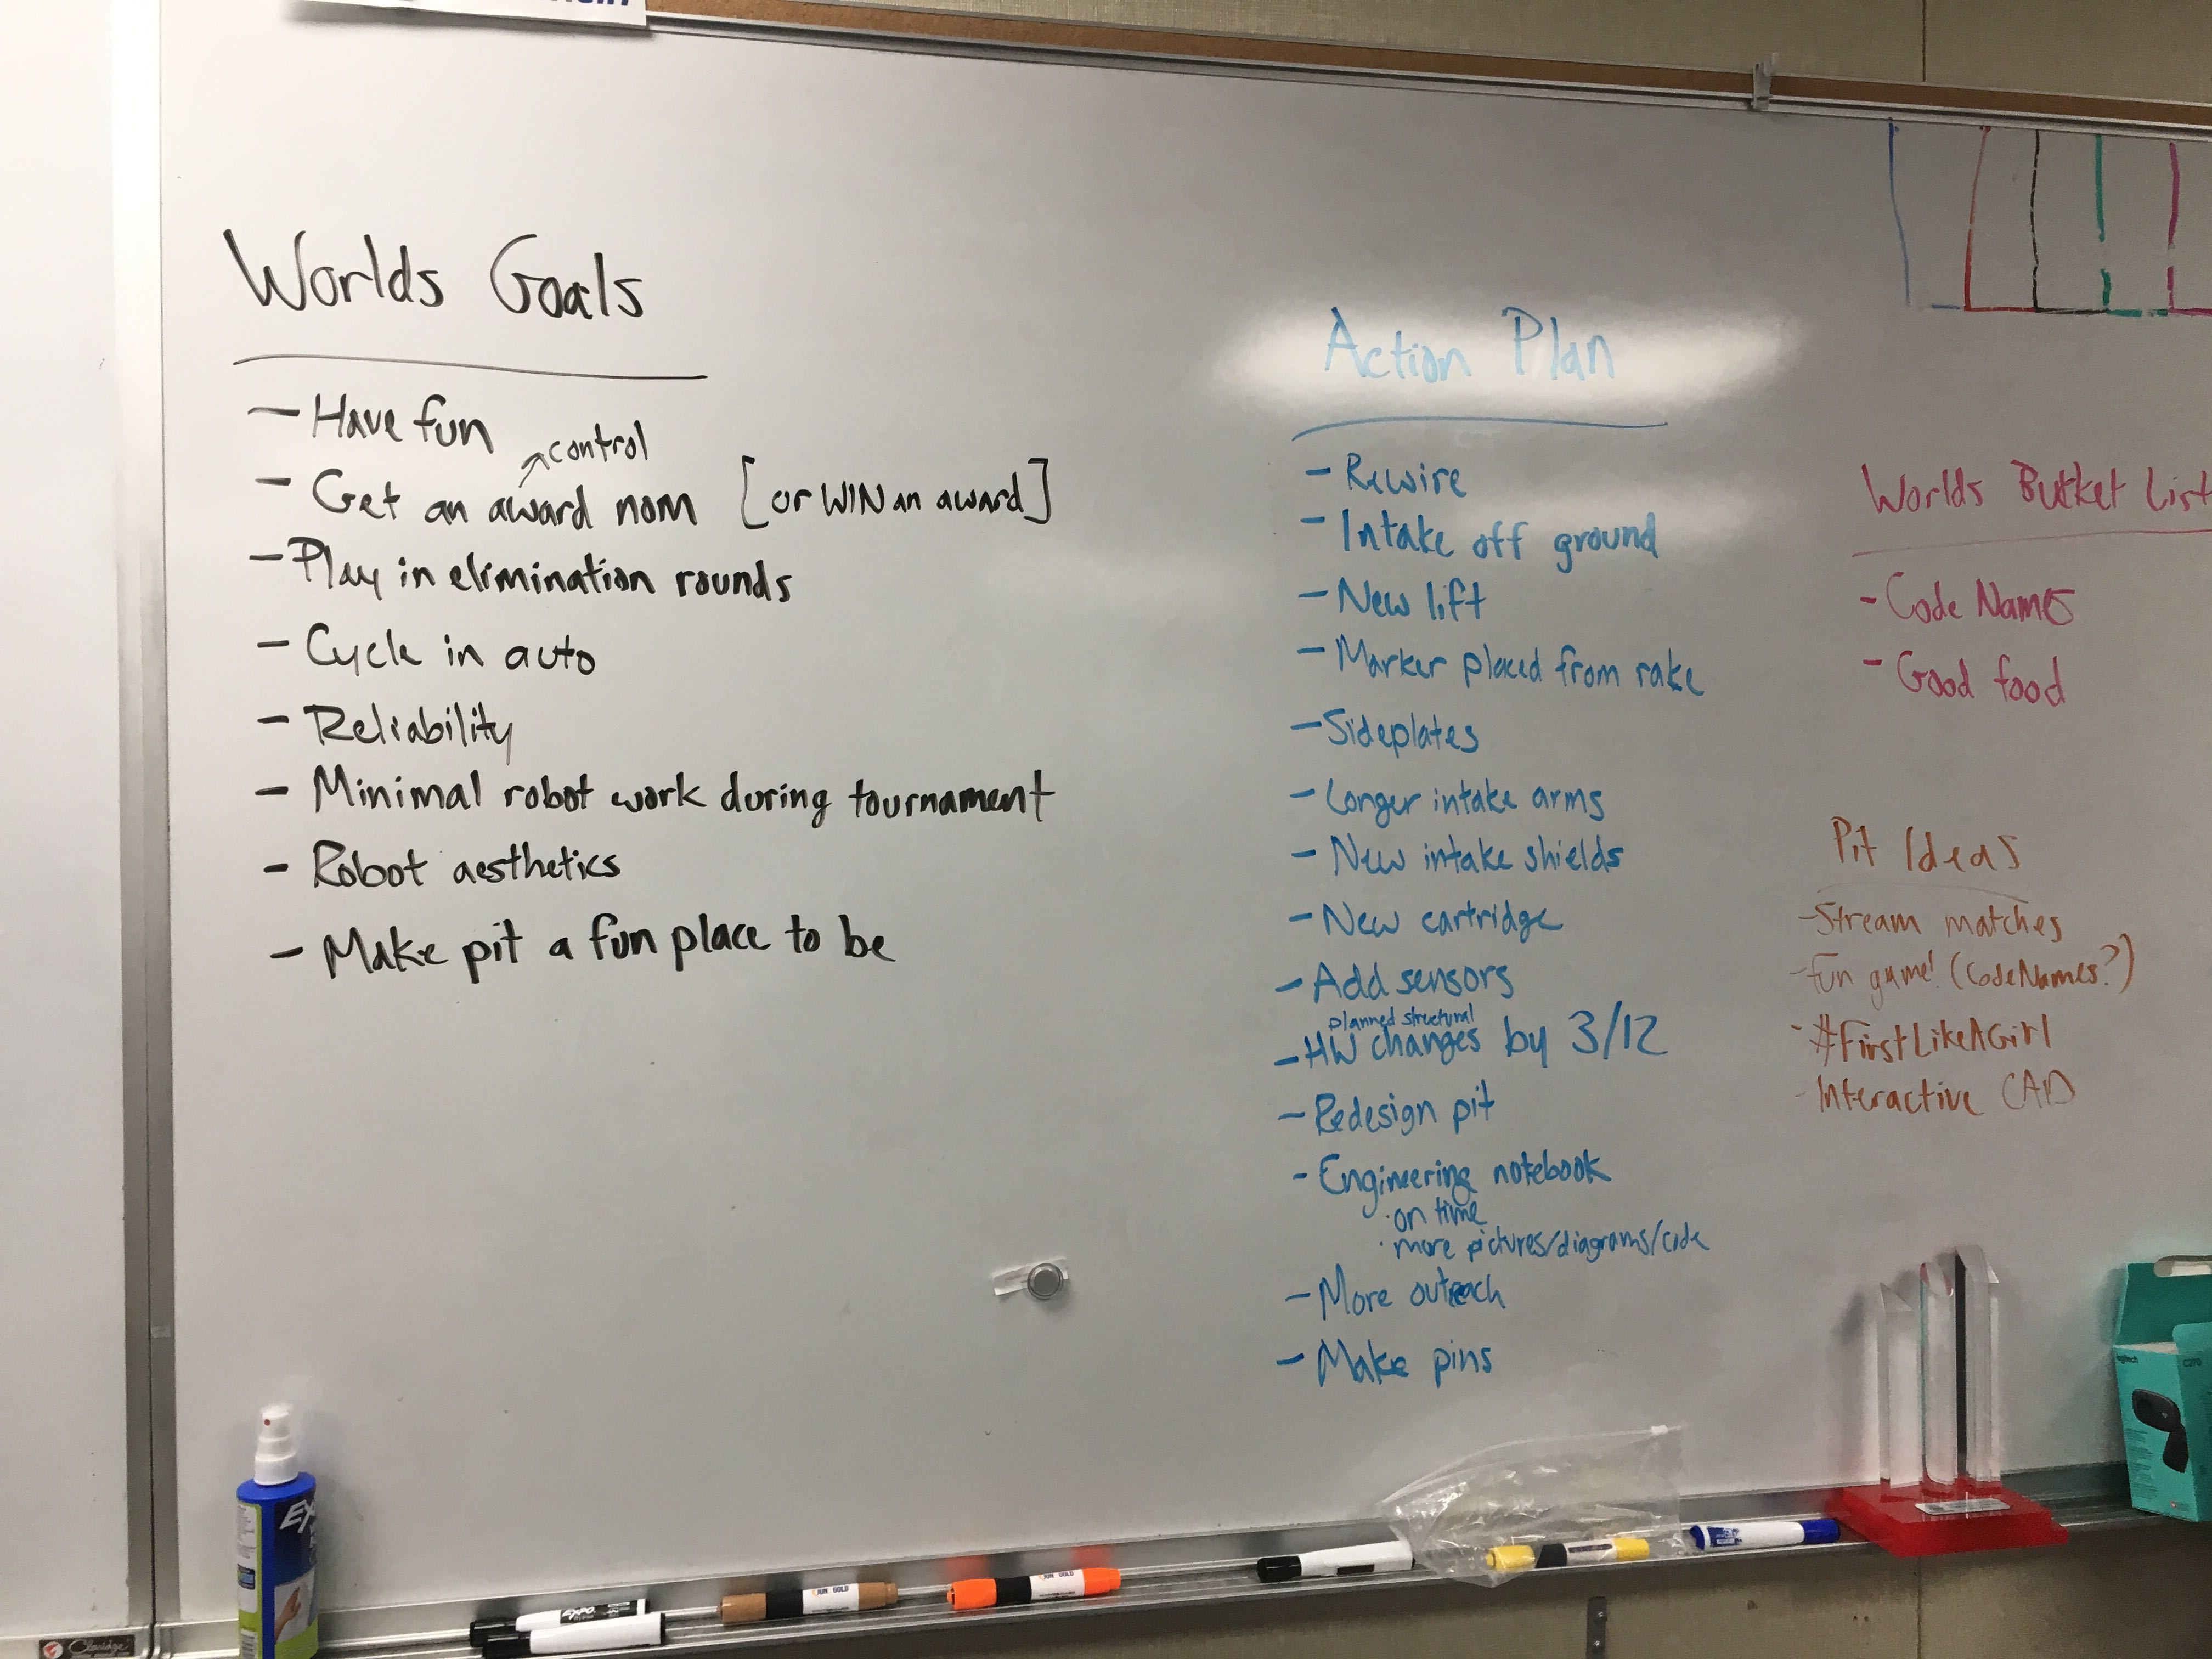
\includegraphics[width= 0.5 \textwidth]{27_03-04/images/goalsandactionplan.JPG}
    \caption{ACME's Goals and Action Plans for Worlds}
    \label{fig:goals}
\end{figure}

Over the next couple of weeks, ACME will be working hard to meet these goals, especially the hardware deadlines and engineering notebook goals. \\

\subsection{Plan outreach events}
ACME had a good section of time between the end of NorCals and Worlds. Since they were planning to have the robot done two weeks after NorCals, they would have four more weeks in which to do software, drive practice, and outreach events. The business team decided that they wanted to put on a few outreach events between now and Worlds. To do this they created a list of possible events and picked a few based off of how doable, fun, and interesting they would be. Here are the outreach events they were considering:

\begin{itemize}
    \item Hackathon
    \item Host a movie night
    \item Girl Scout Workshop
    \item Expert Consultations
    \item Vex Team Meet-Up
\end{itemize}

The team decided that a Hackathon sounded like something that could easily be done in the time span they had, and it seemed like a lot of fun. ACME has a connection with a member of the local Economic Resource Council, who recently hosted Hackathon for adults. The team asked Shavati Karki-Pearl if the ERC, specifically the Nevada County Tech Connection, would want to work with ACME to put on a shorter Hackathon for middle and high schoolers. She said that would be doable and agreed to work with the team! This week, ACME planned out the basic outline of how the day will go. Emma and Kelly decided the Hackathon would be 8 hours long, as they felt even that would be a very long time for the students to be focused on their task. It will be held at the ERC room in Nevada City. The ERC generously decided to provide lunch for the event. The team is planning on having the students bring their own computers, but will have a few of theirs in reserve just in case. Students do not have to have any coding experience to attend, in fact, ACME is planning on giving a hour long workshop using Scratch at the beginning of the day. Students will be working in groups to program a video game using Scratch, Java, JavaScript, Python, or whatever coding language they are familiar with or choose. Although they have not settle on a date yet, the event will take place sometime at the end of March or beginning of April. \\

Another idea the team had was to invite business professionals from their sponsoring companies to give them advice on areas they needed improvement on. They decided to called this series of speakers their "expert consultations". ACME already has a meeting lined up with an employee at Telestream who is very well versed in color-spaces. The software team was working on developing mineral detection and thought that he could give them some advice on how to accomplish that. \\

There is also the possibility of hosting and running another Girl Scouts workshop with another Girl Scouts troop. This will be great to do as the team already has one workshop under their belts. With a few improvements, the team could give a fairly comprehensive workshop for the girls by teaching them how to use the LEGO Mindstorms kits and software. \\

All of these events will hopefully take place in the gap between the time of this entry and Worlds. ACME is really excited to start working on these events. \\

\end{document}